\documentclass[a4paper,10pt,oneside]{amsart}
\usepackage{latexsym}
\usepackage{amsmath}
\usepackage{amsfonts}
\usepackage{amsthm}
\usepackage{amssymb}
\usepackage{fncylab}
\usepackage{tikz}
\usepackage{url}
\usepackage[margin=1cm]{geometry}
\usetikzlibrary{decorations.fractals,chains,fit,shapes}
\usepackage{tikz}
\usepackage{tikz-qtree}
\include{pythonlisting}
\usepackage[utf8]{inputenc}
\relpenalty=9999
\binoppenalty=9999


%----------definitions---------------------------


%math definitions

\newcommand{\R}{\mathbb R}
\newcommand{\C}{{\mathcal C}}
\newcommand{\F}{{{\mathcal F}}}
\newcommand{\U}{{{\mathcal U}}}
\newcommand{\V}{{{\mathcal V}}}
\newcommand{\cont}{{\mathfrak{c}}}
\newcommand{\force}{\Vdash}
\newcommand{\pw}{{{\mathcal P}}}
\newcommand{\MU}{{\mathbb{M}_{\mathcal{U}}}}
\newcommand{\pomega}{\pw(\omega)}






%---------numbering of the theorems------------
 \swapnumbers

 \newtheorem*{theorem*}{Theorem}
 \newtheorem{theorem}[subsection]{Theorem}
 \newtheorem{proposition}[subsection]{Proposition}
 \newtheorem{observation}[subsection]{Observation}
 \newtheorem{fact}[subsection]{Fact}
 \newtheorem{lemma}[subsection]{Lemma}
 \theoremstyle{definition}
 \newtheorem{definition}[subsection]{Definice}
 \newtheorem{ukol}{Úloha}
 \newtheorem{pozn}[subsection]{Pozn.}
 \newtheorem*{pozn*}{Pozn}
 \newtheorem*{definition*}{Definice}
 \newtheorem*{question*}{Question}
 \newtheorem{notation}[subsection]{Notation}
 \newtheorem{remark}[subsection]{Remark}
 \newtheorem*{note}{Note}
 \newtheorem*{ack}{Acknowledgements}
 
\pdfinfo{
     /Author ()
     /Title ()
     /Subject (2010 MSC: Primary )
     /Keywords ()
  }


%-------------opening--------------------------
\begin{document}
\title{}

% \author{Jonathan Verner}
% \address{Department of Logic, Charles University\\
% Palachovo nám. 2\\ 116 38 Praha 1, Czech Republic}
\email{jonathan.verner{@}ff.cuni.cz}
%\thanks{The author was partially supported by }

%\subjclass[2010]{Primary }
%\keywords{}

%\begin{abstract}
%\end{abstract}
%\maketitle
\thispagestyle{empty}
\section*{Cvičení 10. dubna 2012}
%\hsize=16cm
\parindent=0cm

{\it 
Cílem tohoto úkolu je napsat program, který setřídí zadaný soubor a uloží výsledek do jiného souboru.
Třídícím algoritmem bude buď Quicksort nebo Heapsort. Níže si v krátkosti připomeneme jak oba algoritmy
fungují.}

\medskip

{\bf Quicksort} je klasickým rekurzivním algoritmem (nebo také ``rozděl a panuj''). Funguje na
následujícím principu. Pokud má seznam, který se má setřídit, pouze jeden prvek, je setřízený a algoritmus
může skončit. V opačném případi si seznam rozdělí na dvě části tak, aby všechny položky v levé části byly 
menší než všechny položky v pravé části. Pak se rekurzivně zavolá a setřídí
levou a pravou část. Následně může prostě připojit setřízenou pravou část za setřízenou levou část
a celý seznam bude setřízený, protože prvky v levo byly menší než prvky v pravo a obě části setřízené
byly. Zbývá popsat rozdělování na části. To se typicky provádí tak, že se ze seznamu náhodně zvolí jeden
prvek, tzv. \emph{pivot}, a pole se rozdělí tak, aby vlevo byly všechny prvky menší nebo rovné pivotu
a v pravo všechny prvky větší nebo rovné pivotu. Seznamem se prochází současně zleva i zprava. V okamžiku, kdy z 
jednoho směru narazíme na prvek, který má být vzhledem k pivotu v opačné části, čekáme, než k takovému
prvku dorazíme i zprava (pokud na žádný nenarazíme, víme, že jsme hotovi a tento prvek bude první prvek,
který patří do pravé části). V okamžiku, kdy na takový prvek narazíme i zprava, oba prvky vyměníme
a pokračujeme. Když se setkáme, máme pole rozdělené. Schematicky bude quicksort vypadat takto:

\begin{python}
def quicksort( seznam ):
    if len(seznam) == 1:
      return seznam
    pivot = zvol_pivota( seznam )
    L, P = rozdel_seznam( seznam, pivot )
    L_sorted = quicksort(L)
    P_sorted = quicksort(P)
    return L_sorted + P_sorted
\end{python}

\begin{pozn*} Ve skutečnosti by výše uvedený schematicky zapsaný quicksort byl relativně pomalý,
protože by docházelo k častému kopírování z paměti do paměti při vytváření nových polí (L,P, L+P).
Ve vašem řešení proto vůbec nebudete vytvářet nové seznamy, nýbrž vaše funkce bude vypadat spíše
takto:
\begin{python}
def quicksort( seznam, start, end ):
    if start >= end:
        # Prazdne a jednoprvkove pole jsou
        # z definice setrizne
        return  
    pivot = zvol_pivota( seznam, start, end )
    stred = rozdel_seznam( seznam, start, end, pivot)
    quicksort( seznam, start, stred )
    quicksort( seznam, stred+1, end )
    return
\end{python}
t.j. všechno se bude odehrávat v poli {\tt seznam}, nic se nebude nikam kopírovat a podseznamy budou
vždy určené počátečním ({\tt start}) a koncovým indexem ({\tt end}).
\end{pozn*}

\begin{pozn*} Při rozdělování pole je třeba dát pozor na to, aby se pole opravdu ``rozdělilo'', t.j.
aby bylo {\tt start <= stred < end}. Pokud by totiž pravá nebo levá část byla prázdná, program 
by se zacyklil. Tuto podmínku nicméně není těžké splnit, protože pivot může být prvkem jak pravé,
tak levé části.
\end{pozn*}

\medskip

{\bf Heapsort} je algoritmus založný na datové struktuře, které se říká \emph{halda} (angl. \emph{heap}).
Funguje tak, že se celé pole postupně vloží na haldu a pak se z haldy odebírá vrchní prvek a vkládá zpátky do
seznamu. Výsledný seznam bude setřízený, protože vrchní prvek haldy je vždy menší než všechny ostatní prvky
v haldě. K pochopení tohoto algoritmu je tedy potřeba pochopit jak funguje halda. Halda je speciální případ
binárního stromu, ve kterém je v každém uzlu navíc uložen nějaký prvek. Jakožto strom je to strom, ve kterém
se každý uzel, který není listem, větví a všechny listy jsou na poslední nebo předposlední hladině s tím, že listy
na poslední hladině jsou ``co nejvíce vlevo''. Prvky, které jsou uložené v uzlech navíc mají tu vlastnost,
že jsou menší než prvky uložené v jejich potomcích. Příkladem haldy je například následující strom:
\begin{center}
\Tree [.2 [.10 [.11 ] [.10 ] ] [.20 ] ]
\end{center}

Naopak ani jeden z následujících stromů haldou není.
\begin{center}
(A)
\begin{minipage}{4cm}
\Tree [.0 [.10 [.11 ] [.9 ] ] [.20 ] ] 
\end{minipage}
(B)
\begin{minipage}{6cm}
\Tree [.0 [.10 [.11 [.15 ] [.16 ] ] [.9 ] ] [.20 [.30 [.35 ] [.37 ] ] [.31 [.32 ] [.33 ] ] ] ]
\end{minipage}
(C)
\begin{minipage}{4cm}
\Tree [.0 [.10 [.11 ] [.9 ] ] ]
\end{minipage}
\end{center}
Ve stromu (A) je porušena podmína, že uzly jsou menší než jejich potomci ($10\not\leq 9$), ve stromu (B) je
porušena podmínka, že listy na poslední hladině mají být úplně vlevo a ve stromu (C) je porušena podmínka,
že každý uzel, který není listem, se musí větvit.

Prvky se do haldy přidávají tak, že se vytvoří nový list a do něj se prvek vloží. Tím může dojít k porušení
podmínky, že uzly jsou menší než potomci. Proto musíme zkontrolovat, zda je vložený prvek větší než jeho rodič.
Pokud není, s rodičem ho vyměníme a musíme dále zkontrolovat rodiče s jeho rodičem. Pokud je vše O.K., skončíme,
jinak pokračujeme v prohazovaní dokud se nedostaneme do kořene, který žádného rodiče nemá.

Příklad přidávání prvku $1$ do haldy:

\begin{center}
\begin{minipage}{4cm}
\Tree [.2 [.10 [.11 ] [.10 ] ] [.20 ] ]
\end{minipage}
$\Rightarrow$
\begin{minipage}{4cm}
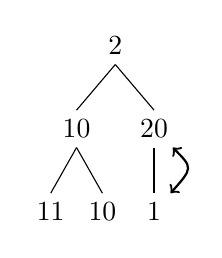
\begin{tikzpicture}
\Tree [.2 [.10 [.11 ] [.10 ] ] [.\node(a){20}; [.\node(b){1}; ] ] ]
\draw[thick,<->](a)..controls +(south east:0.7).. (b);
\end{tikzpicture}
\end{minipage}
$\Rightarrow$
\begin{minipage}{4cm}
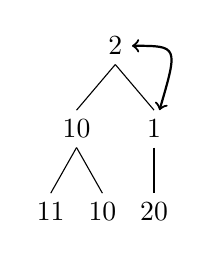
\begin{tikzpicture}
\Tree [.\node(a){2}; [.10 [.11 ] [.10 ] ] [.\node(b){1}; [.20 ] ] ]
\draw[thick,<->](a)..controls +(east:0.8).. (b);
\end{tikzpicture}
\end{minipage}
$\Rightarrow$
\begin{minipage}{4cm}
\Tree [.1 [.10 [.11 ] [.10 ] ] [.2 [.20 ] ] ]
\end{minipage}
\end{center}

Naopak z hlady se (vrchní) prvek odebírá tak, že se vrátí hodnota v kořeni a nahradí se hodnotou v nejpravějším
listu na poslední hladině a tento list se smaže. Tím může být opět porušeno pravidlo, že uzly jsou menší než následníci, proto musíme zkontrolovat, zda
nová hodnota kořene je větší než hodnota obou jeho dětí. Pokud není, vyměníme tuto hodnotu s hodnotou menšího
dítěte a pokračujeme v kontrolování tohoto dítěte dokud není vše O.K., nebo dokud se nedostaneme do listu, kde
je vše O.K. z definice.

\begin{center}
\begin{minipage}{4cm}
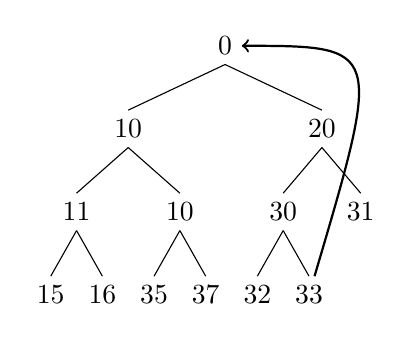
\begin{tikzpicture}
\Tree [.\node(a){0}; [.10 [.11 [.15 ] [.16 ] ] [.10 [.35 ] [.37 ] ] ] [.20 [.30 [.32 ] [.\node(b){33}; ] ] [.31 ] ] ]
\draw[thick,<-](a)..controls +(east:2).. (b);
\end{tikzpicture}
\end{minipage}
$\Rightarrow$
\begin{minipage}{4cm}
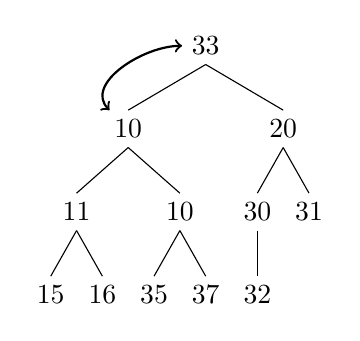
\begin{tikzpicture}
\Tree [.\node(a){33}; [.\node(b){10}; [.11 [.15 ] [.16 ] ] [.10 [.35 ] [.37 ] ] ] [.20 [.30 [.32 ] ] [.31 ] ] ]
\draw[thick,<->](a)..controls +(west:0.8) and +(north west:0.8) .. (b);
\end{tikzpicture}
\end{minipage}
$\Rightarrow$
\begin{minipage}{4cm}
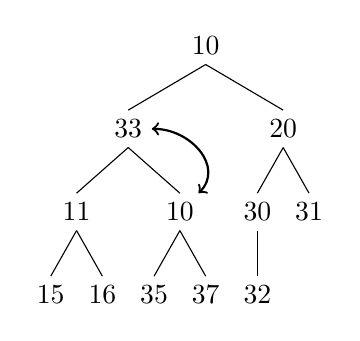
\begin{tikzpicture}
\Tree [.10 [.\node(a){33}; [.11 [.15 ] [.16 ] ] [.\node(b){10}; [.35 ] [.37 ] ] ] [.20 [.30 [.32 ] ] [.31 ] ] ]
\draw[thick,<->](a)..controls +(east:0.8) and +(north east:0.8) .. (b);
\end{tikzpicture}
\end{minipage}
$\Rightarrow$
\begin{minipage}{4cm}
\Tree [.10 [.10 [.11 [.15 ] [.16 ] ] [.33 [.35 ] [.37 ] ] ] [.20 [.30 [.32 ] ] [.31 ] ] ]
\end{minipage}
\end{center}

\medskip

Zbývá ještě vyřešit otázku, jak v programu haldu reprezentovat. Haldu lze reprezenovat stejně, jako by se reprezentoval strom,
nicméně pro účely třízení je lepší ji mít uloženou v poli a využít vlastnosti hlady, která nám umožní z indexu uzlu spočítat
index jeho rodiče i jeho dětí. Uzly v hladě očíslujeme postupně po hladinách zleva do prava. Na následujícím obrázku je příklad
očíslované haldy (očíslování je uvedeno v horních indexech) a její reprezentaci v poli:

\begin{center}
\begin{minipage}{15cm}
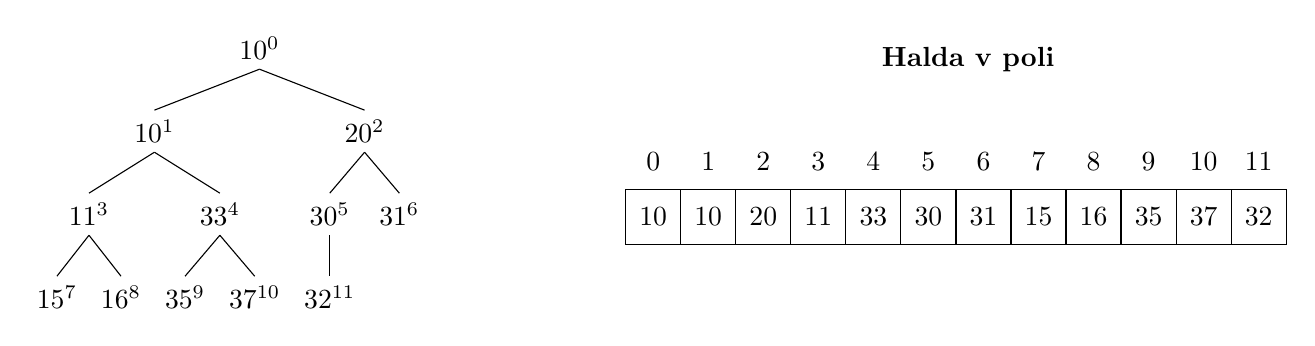
\begin{tikzpicture}
\Tree [.{$10^0$} [.{$10^1$} [.{$11^3$} [.{$15^7$} ] [.{$16^8$} ] ] [.{$33^4$} [.{$35^9$} ] [.{$37^{10}$} ] ] ] [.{$20^2$} [.{$30^5$} [.{$32^{11}$} ] ] [.{$31^6$} ] ] ]
\tikzstyle{tmtape}=[draw,minimum size=0.7cm]
\tikzstyle{arrayindex}=[minimum size=0.7cm]
\begin{scope}[start chain=1 going right,node distance=-0.15mm,shift={(5cm,-2cm)}]
    \node [on chain=1,tmtape] {10};
    \node [on chain=1,tmtape] (input) {10};
    \node [on chain=1,tmtape] {20};
    \node [on chain=1,tmtape] {11};
    \node [on chain=1,tmtape] {33};
    \node [on chain=1,tmtape] {30};
    \node [on chain=1,tmtape] {31};
    \node [on chain=1,tmtape] {15};
    \node [on chain=1,tmtape] {16};
    \node [on chain=1,tmtape] {35};
    \node [on chain=1,tmtape] {37};
    \node [on chain=1,tmtape] {32};
\end{scope}
\begin{scope}[start chain=2 going right,node distance=-0.15mm,shift={(5cm,-1.3cm)}]
    \node [on chain=2,arrayindex] {0};
    \node [on chain=2,arrayindex] (input) {1};
    \node [on chain=2,arrayindex] {2};
    \node [on chain=2,arrayindex] {3};
    \node [on chain=2,arrayindex] {4};
    \node [on chain=2,arrayindex] {5};
    \node [on chain=2,arrayindex] {6};
    \node [on chain=2,arrayindex] {7};
    \node [on chain=2,arrayindex] {8};
    \node [on chain=2,arrayindex] {9};
    \node [on chain=2,arrayindex] {10};
    \node [on chain=2,arrayindex] {11};
\end{scope}
\begin{scope}[shift={(9cm,0cm)}]
\node {\textbf{Halda v poli}}; 
\end{scope}
\end{tikzpicture}
\end{minipage}
\end{center}

Všimněte si nyní, že je-li $u$ index uzlu, pak index jeho rodiče dostaneme jako $\lfloor{(u-1)/2}\rfloor$,
zatímco index jeho levého dítěte je $2u+1$ a index jeho pravého dítěte je $2u+2$.

\end{document}
